% !TEX TS-program = pdflatexmk
\documentclass[12pt]{article}

% Layout.
\usepackage[top=1in, bottom=0.75in, left=1in, right=1in, headheight=1in, headsep=6pt]{geometry}

% Fonts.
\usepackage{mathptmx}
\usepackage[scaled=0.86]{helvet}
\renewcommand{\emph}[1]{\textsf{\textbf{#1}}}
\newcommand{\ans}[1][1in]{\rule{#1}{.5pt}}

\usepackage[parfill]{parskip}

% Misc packages.
\usepackage{amsmath,amssymb,latexsym}
\usepackage{graphicx,hyperref}
\usepackage{array}
\usepackage{xcolor}
\usepackage{multicol,tikz}
\usetikzlibrary{calc, positioning}
\usepackage{tabularx,colortbl,booktabs,xparse}
\usepackage{enumitem}

% Rotation: \rot[<angle>][<width>]{<stuff>}
\NewDocumentCommand{\rot}{O{45} O{1em} m}{\makebox[#2][l]{\rotatebox{#1}{#3}}}%

\usepackage{fancyhdr}
\pagestyle{fancy} 
\lhead{\large\sf\textbf{MATH F113X: Euler Paths and Circuits}}
%\chead{\large\sf\textbf{lecture notes}}
%\rhead{\large\sf\textbf{Day 1}}

\begin{document}

\emph{Terminology}: Euler Path (a.k.a Eulerian Path), Euler Circuit (a.k.a. Eulerian circuit)

Konigsberg and Leonhard Euler [``oiler'']

\includegraphics[width = .5\linewidth]{BookEulerPic.jpg}

\emph{Euler Path}

\vfill

\emph{Euler Circuit}

\vfill

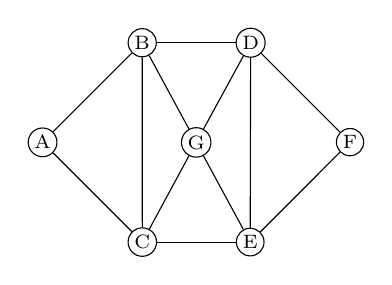
\begin{tikzpicture}[vtx/.style = {draw, circle, inner sep = 1pt, font = \scriptsize}]
\node[vtx](A) at (0,0){A};
\node[vtx, above right = of A] (B) {B};
\node[vtx, below right = of A] (C) {C};
\node[vtx, right = of B] (D) {D};
\node[vtx, right = of C] (E) {E};
\node[vtx, below right = of D] (F) {F};
\node[vtx] (G) at ($(B)!.5!(E)$) {G};
\foreach  \i/\j in {
A/B, B/D, D/F,  B/G, D/G, G/C, G/E, C/E, B/C, D/E, F/E, A/C}{
\draw (\i) -- (\j);
}
\end{tikzpicture}
%%%%%%
\hfill
%%%%%%%%%
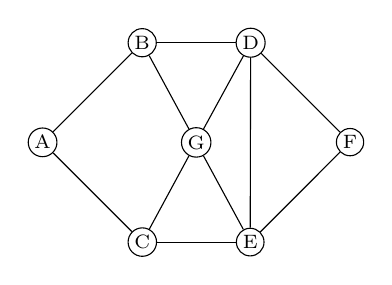
\begin{tikzpicture}[vtx/.style = {draw, circle, inner sep = 1pt, font = \scriptsize}]
\node[vtx](A) at (0,0){A};
\node[vtx, above right = of A] (B) {B};
\node[vtx, below right = of A] (C) {C};
\node[vtx, right = of B] (D) {D};
\node[vtx, right = of C] (E) {E};
\node[vtx, below right = of D] (F) {F};
\node[vtx] (G) at ($(B)!.5!(E)$) {G};
\foreach  \i/\j in {
A/B, B/D, D/F,  B/G, D/G, G/C, G/E, C/E, D/E,  F/E, A/C}{
\draw (\i) -- (\j);
}
\end{tikzpicture}
%%%%%%
\hfill
%%%%%%%%%
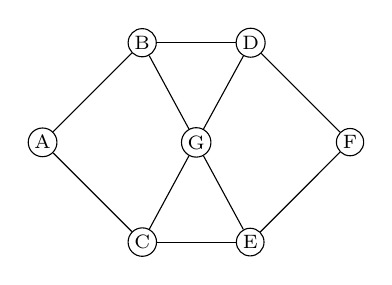
\begin{tikzpicture}[vtx/.style = {draw, circle, inner sep = 1pt, font = \scriptsize}]
\node[vtx](A) at (0,0){A};
\node[vtx, above right = of A] (B) {B};
\node[vtx, below right = of A] (C) {C};
\node[vtx, right = of B] (D) {D};
\node[vtx, right = of C] (E) {E};
\node[vtx, below right = of D] (F) {F};
\node[vtx] (G) at ($(B)!.5!(E)$) {G};
\foreach  \i/\j in {
A/B, B/D, D/F,  B/G, D/G, G/C, G/E, C/E, F/E, A/C}{
\draw (\i) -- (\j);
}
\end{tikzpicture}

\vfill

\emph{Applications}

\vfill

%\newpage


\end{document}